\section{Monte Carlo event generation}
\label{sec:mc}


We used the external model interface in MadGraph~\cite{madgraph} 
to generate $pp \to tt$ and $pp \to ttj$ at LO 
using the lagrangian of equation 1 with
different values of 
the $Z'$ mass, and with $f_L = 0$, $f_R = 1$.  We simulated the model
with $Z'$ mass in t- and s-channels ranging from 100 GeV to 2 TeV  and 
between 200 GeV to 2 TeV, respectively. In the s-channel diagram the $Z'$ boson
decays to a top and a light flavour quark. In order to be on-shell
its mass has to be larger than the top mass. Thus, we have used a lower
cutoff of 200 GeV in our simulations.


Different
values of $f_R$ are modelled by rescaling the cross-sections
for the t-channel (Fig.~\ref{fig:tchannel}) and 
s-channel (Fig.~\ref{fig:schannel}) by $f_R^4$ and $f_R^2$,
respectively.  We used the 
CTEQ6L~\cite{cteq6l} parton distribution function (PDF). 
The renormalization and factorization scales are chosen 
to be at the top mass scale ($m_{t} = 172.5$ GeV). 
The width of the $Z'$ boson is computed using 
BRIDGE~\cite{bridge} and verified using MadGraph~\cite{madgraph}. 

The total production cross sections for $tt$ and $ttj$ 
at the leading-order (LO) are shown as a function of $Z'$ 
mass in 
Fig.~\ref{fig:sstopcross}. 
Our calculated cross sections agree well with the 
published literature~\cite{berger}. 

\begin{figure}[htb]
\begin{center}
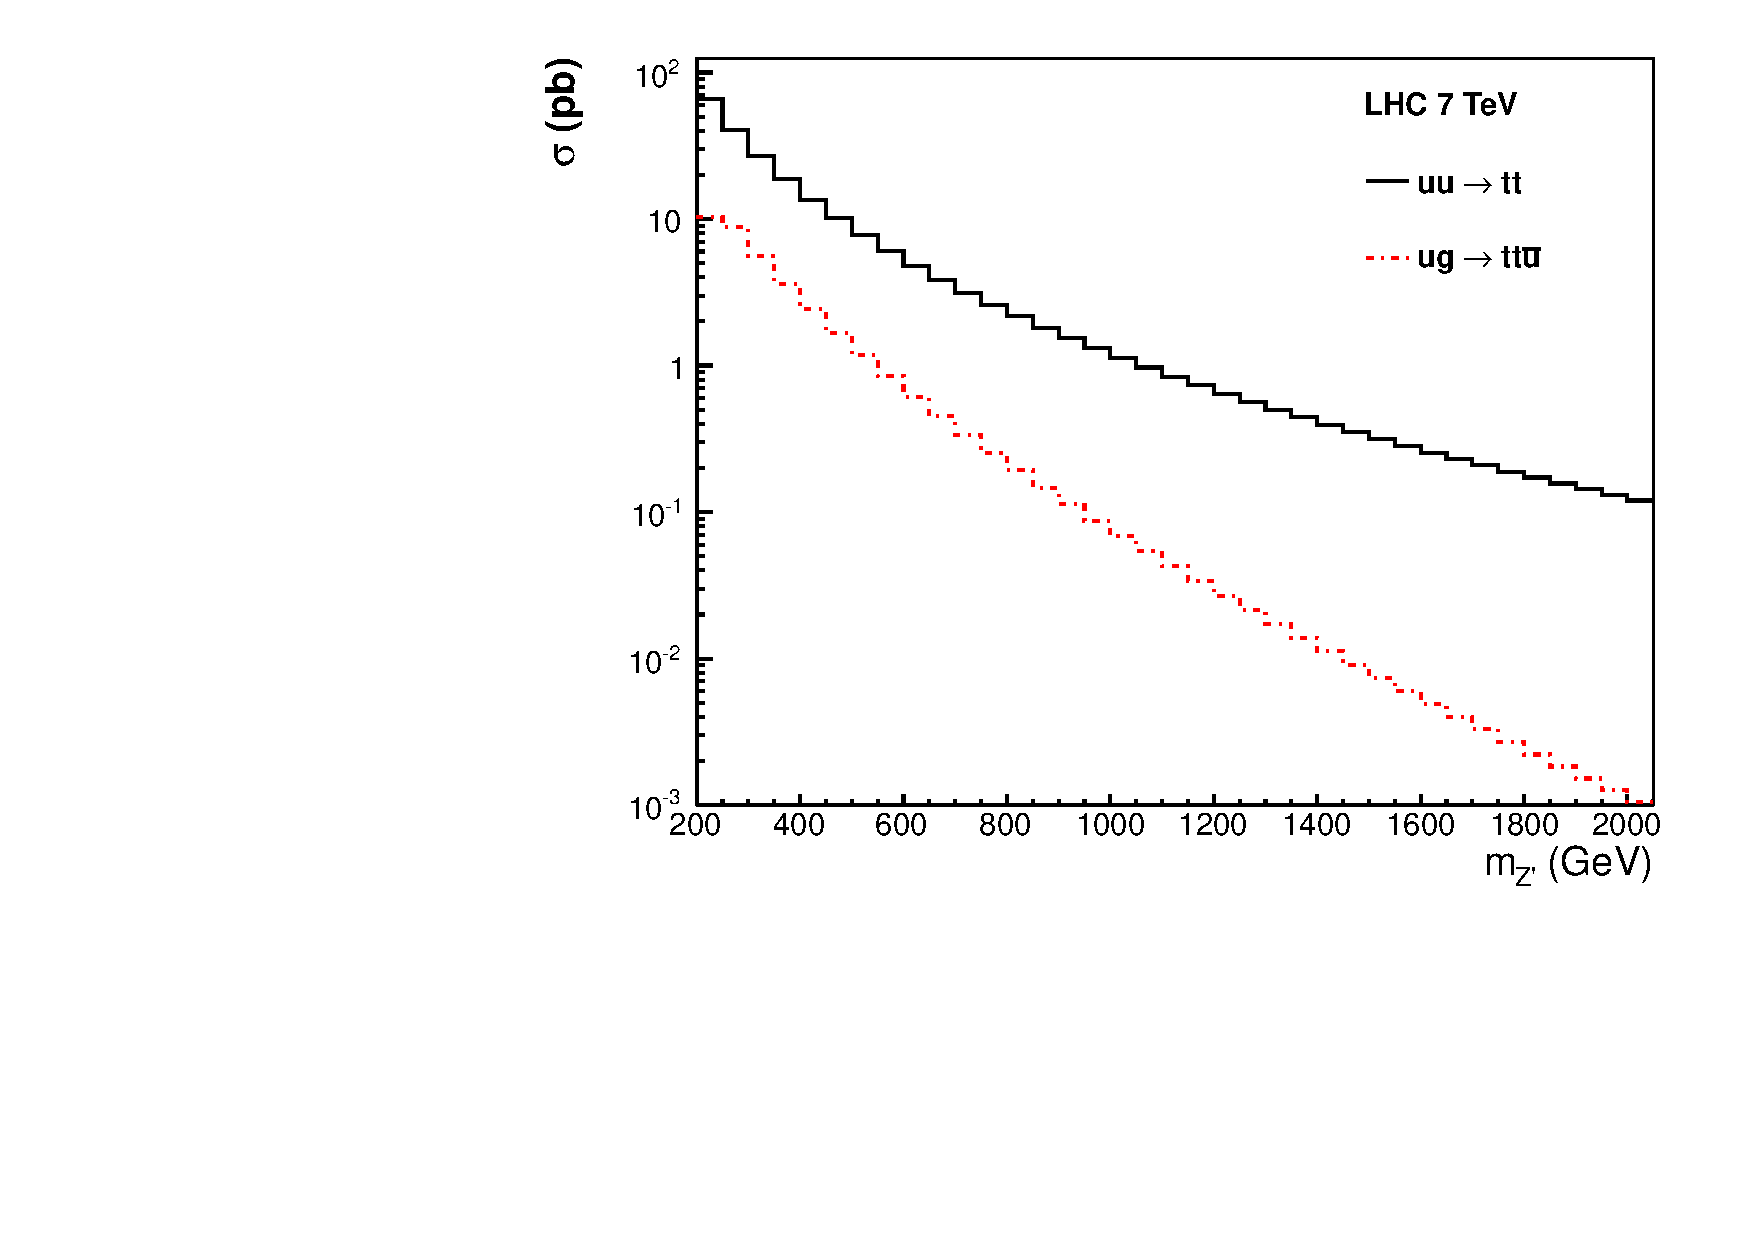
\includegraphics[width=0.7\linewidth]{figs/sstopcross.pdf}
\caption{ LHC production cross section for $tt$ and $ttj$ diagrams using right-handed coupling, $f_R = 1$. 
The renormalization and factorization scales are set to the top mass. \label{fig:sstopcross}}
\end{center}
\end{figure}

The events generated by MadGraph are then fed to Pythia for 
parton showering.  They are simulated using the standard CMS
fast-simulation program.



